\chapter{Results and Discussion}
\label{chap:results and discussion}

This chapter presents the key outcomes obtained during the complete RTL-to-GDSII implementation of the UART IP core. The results include functional verification, synthesis statistics, physical implementation metrics, routing performance, power integrity analysis, physical verification, and the final GDSII layout.

%%%%%%%%%%%%%%%%%%%%%%%%%%%%%%%%%%%%%%%%%%%%%%%%%%%%%%%%%%%%%%%

\section{Functional Verification}

The UART IP core was functionally verified using dedicated Verilog testbenches. The generated simulation waveforms confirm the correct operation of each RTL module before physical implementation.

%%%%%%%%%%%%%%%%%%%%%%%%%%%%%%%%%%%%%%%%%%%%%%%%%%%%%%%%%%%%%%%

\subsection{Baud Rate Generator}

\begin{figure}[!htbp]
\centering
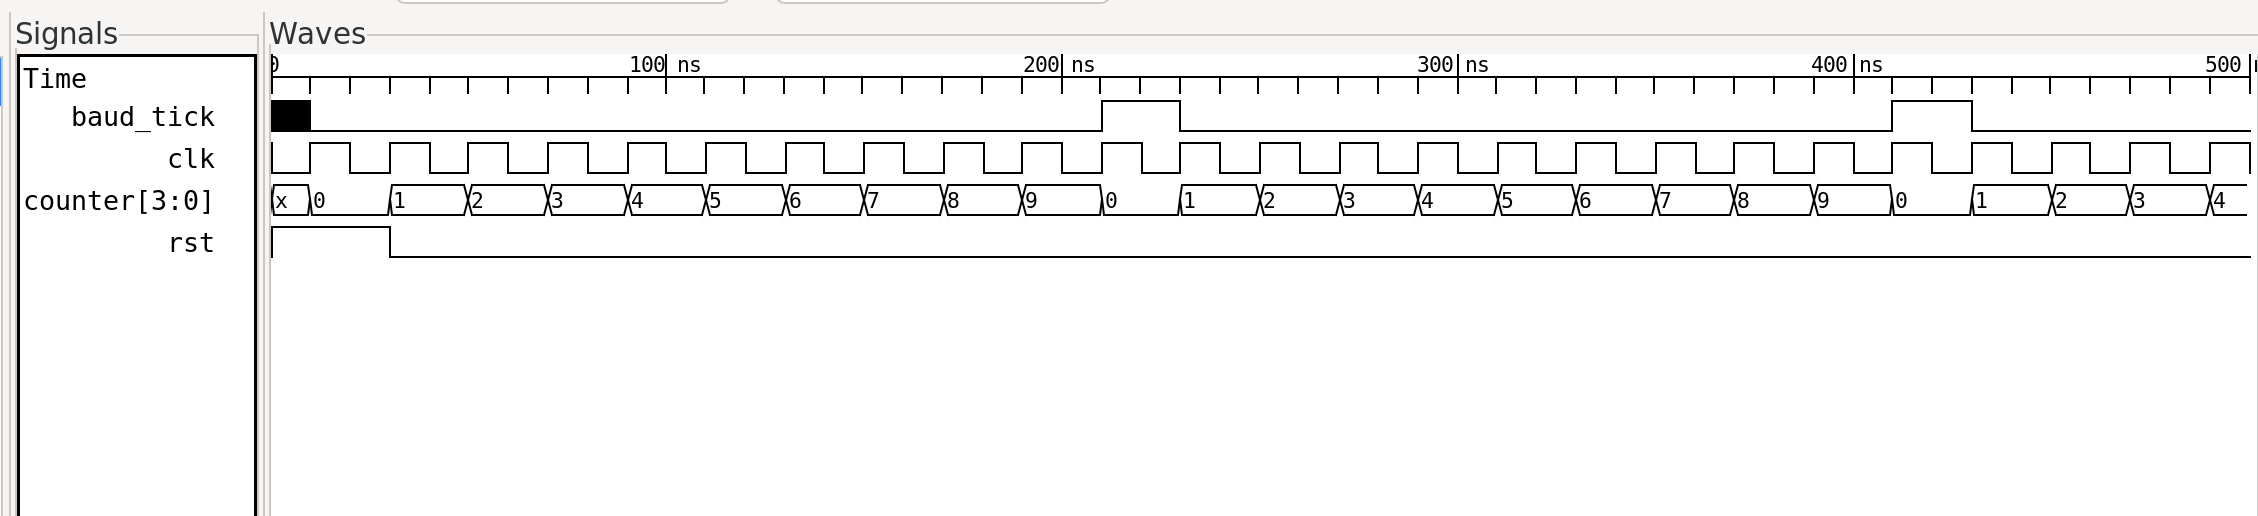
\includegraphics[width=\textwidth]{images/baud_generator_waveform.png}
\caption{Simulation waveform of the Baud Rate Generator.}
\label{fig:baud_wave}
\end{figure}

The waveform verifies that the baud generator correctly divides the system clock and produces periodic baud timing pulses for UART communication.

%%%%%%%%%%%%%%%%%%%%%%%%%%%%%%%%%%%%%%%%%%%%%%%%%%%%%%%%%%%%%%%

\subsection{UART Transmitter}

\begin{figure}[!htbp]
\centering
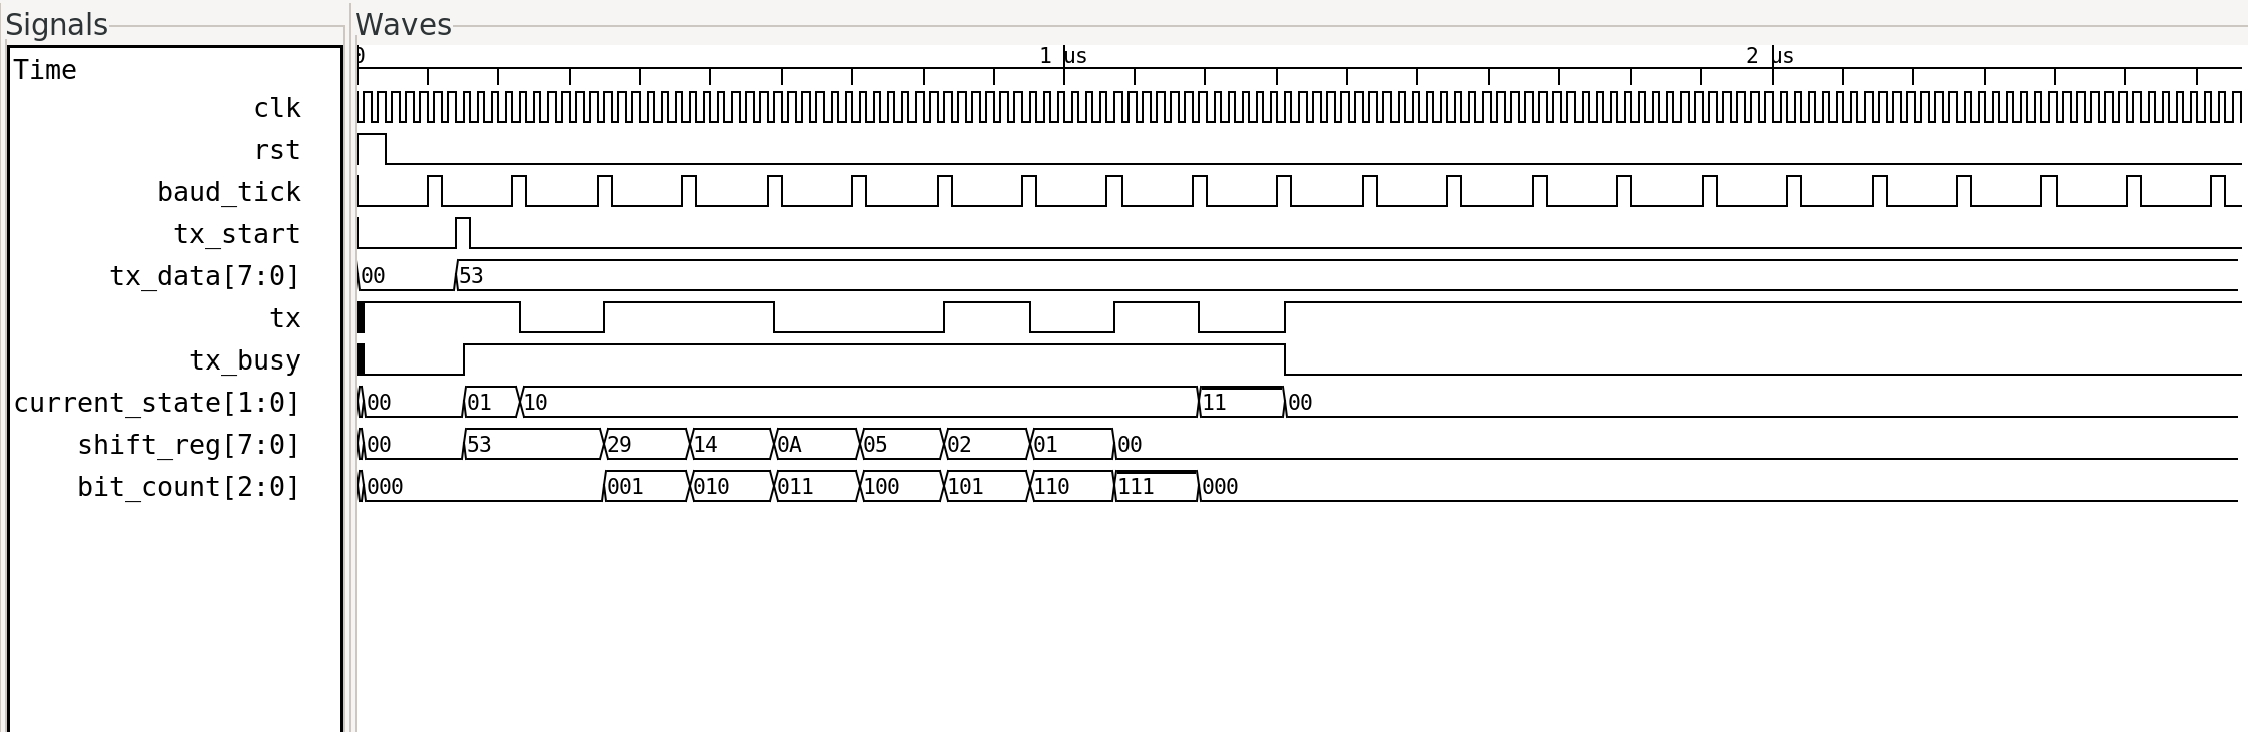
\includegraphics[width=\textwidth]{images/transmitter_waveform.png}
\caption{Simulation waveform of the UART transmitter.}
\label{fig:tx_wave}
\end{figure}

The transmitter correctly generates the UART frame consisting of one start bit, eight data bits, and one stop bit.

%%%%%%%%%%%%%%%%%%%%%%%%%%%%%%%%%%%%%%%%%%%%%%%%%%%%%%%%%%%%%%%

\subsection{UART Receiver}

\begin{figure}[!htbp]
\centering
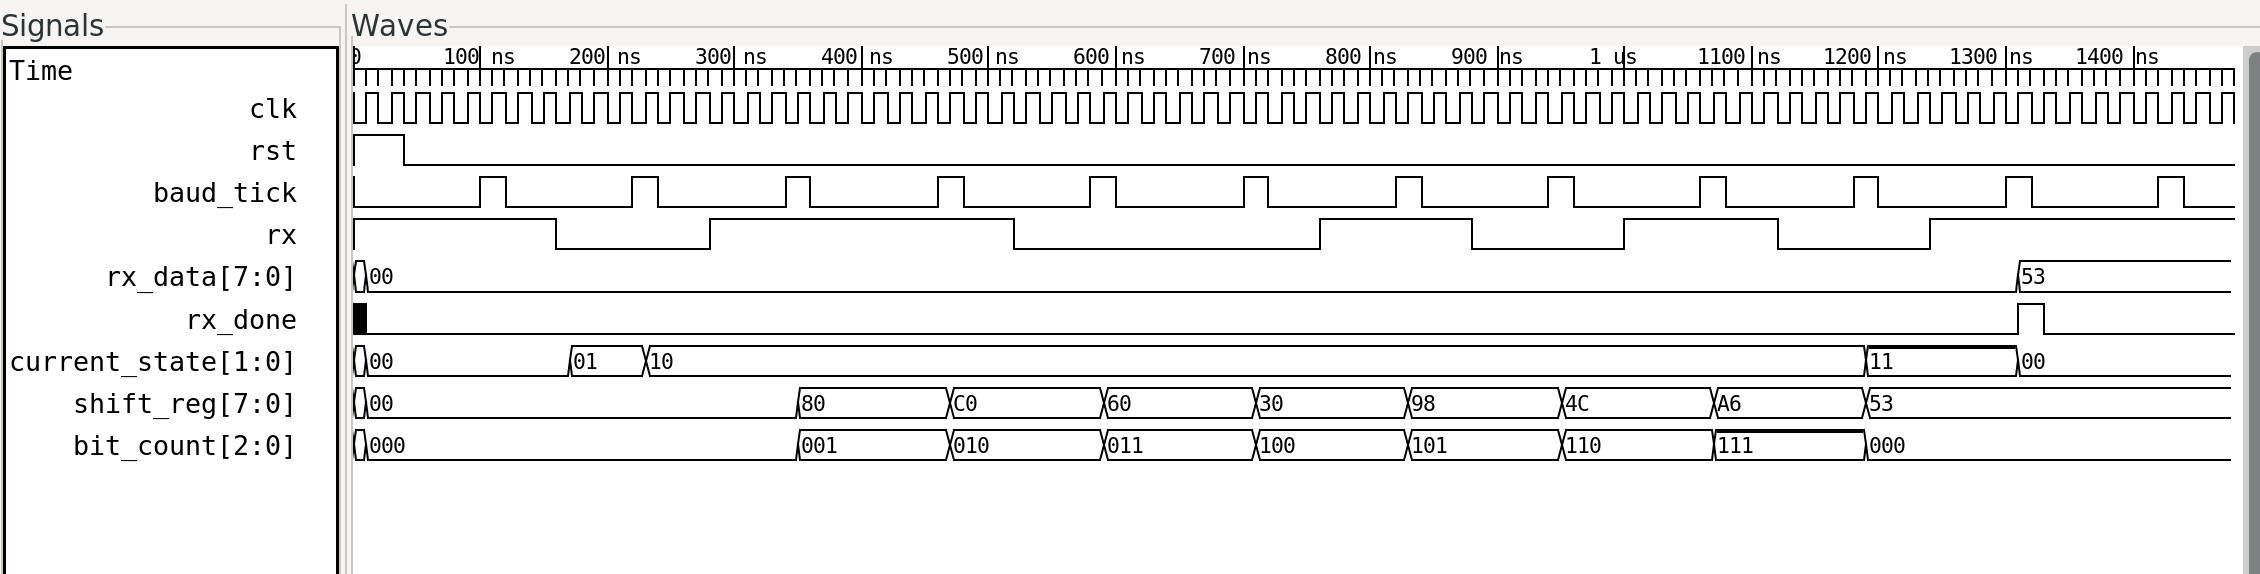
\includegraphics[width=\textwidth]{images/receiver_wavefrom.png}
\caption{Simulation waveform of the UART receiver.}
\label{fig:rx_wave}
\end{figure}

The receiver successfully reconstructs the transmitted serial data and asserts the receive-complete signal after reception.

%%%%%%%%%%%%%%%%%%%%%%%%%%%%%%%%%%%%%%%%%%%%%%%%%%%%%%%%%%%%%%%

\subsection{UART Top Module}

\begin{figure}[!htbp]
\centering
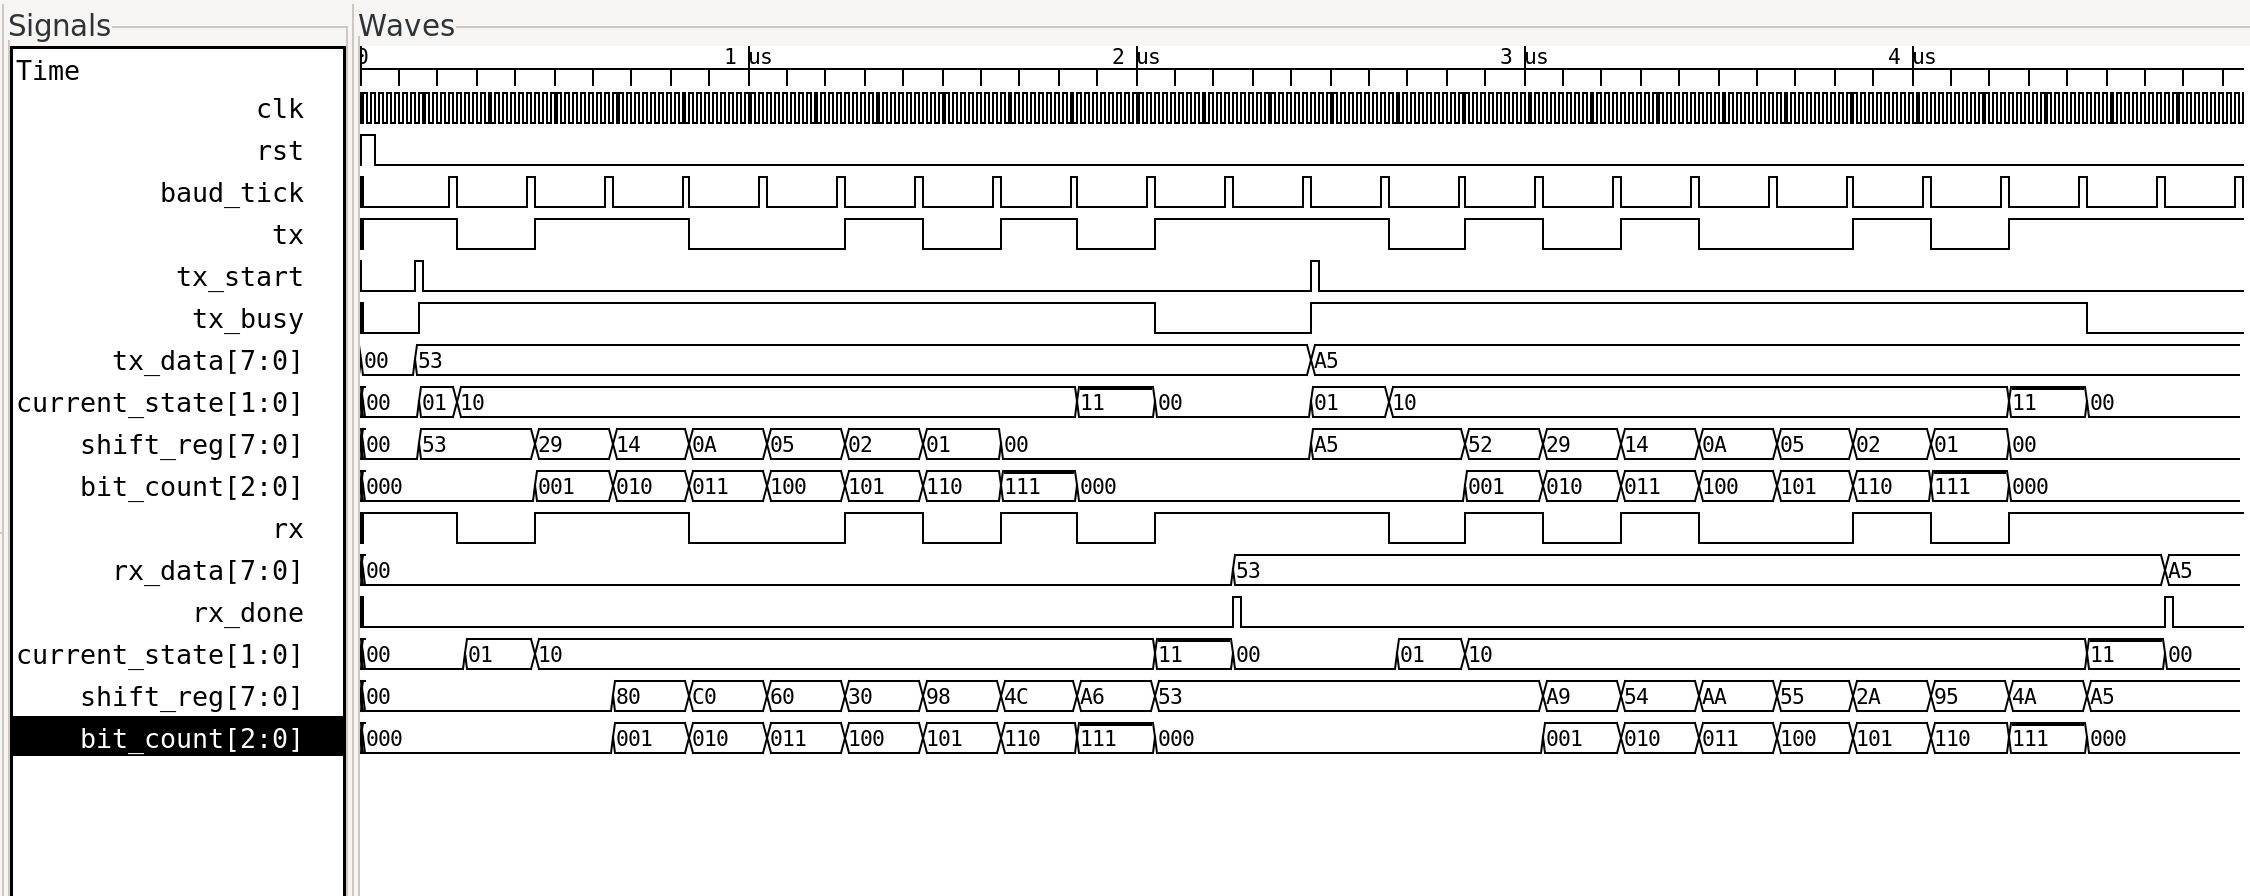
\includegraphics[width=\textwidth]{images/uart_waveform.png}
\caption{Simulation waveform of the complete UART top module.}
\label{fig:top_wave}
\end{figure}

The complete UART system performs successful end-to-end serial communication, confirming proper integration of all RTL modules.

%%%%%%%%%%%%%%%%%%%%%%%%%%%%%%%%%%%%%%%%%%%%%%%%%%%%%%%%%%%%%%%

\section{RTL Synthesis Results}

The RTL was synthesized using Yosys and mapped to the SKY130 standard-cell library.

\begin{table}[!htbp]
\centering
\caption{RTL synthesis summary}
\label{tab:synthesis}
\begin{tabular}{lc}
\toprule
Parameter & Value\\
\midrule
Standard Cells & 219\\
Sequential Cells & 55\\
Cell Area & 2539.936 $\mu m^2$\\
Sequential Area Ratio & 46.06\%\\
Technology Library & SKY130 HD\\
\bottomrule
\end{tabular}
\end{table}

The synthesis completed successfully and generated a technology-mapped gate-level netlist suitable for ASIC implementation.

%%%%%%%%%%%%%%%%%%%%%%%%%%%%%%%%%%%%%%%%%%%%%%%%%%%%%%%%%%%%%%%

\section{Floorplanning Results}

\begin{table}[!htbp]
\centering
\caption{Floorplanning results}
\label{tab:floorplan_result}
\begin{tabular}{lc}
\toprule
Metric & Value\\
\midrule
Die Area & 7658.18 $\mu m^2$\\
Core Area & 5009.80 $\mu m^2$\\
Standard Cell Area & 3210.58 $\mu m^2$\\
Core Utilization & 64.09\%\\
Design Instances & 375\\
I/O Pins & 25\\
\bottomrule
\end{tabular}
\end{table}

The generated floorplan provides sufficient whitespace for routing while maintaining efficient silicon utilization.

%%%%%%%%%%%%%%%%%%%%%%%%%%%%%%%%%%%%%%%%%%%%%%%%%%%%%%%%%%%%%%%

\section{Placement Results}

\begin{table}[!htbp]
\centering
\caption{Placement statistics}
\label{tab:placement_result}
\begin{tabular}{lc}
\toprule
Metric & Value\\
\midrule
HPWL Before Optimization & 3351.5 $\mu m$\\
HPWL After Optimization & 3207.2 $\mu m$\\
HPWL Improvement & 4.3\%\\
Total Displacement & 0 $\mu m$\\
Average Displacement & 0 $\mu m$\\
Maximum Displacement & 0 $\mu m$\\
\bottomrule
\end{tabular}
\end{table}

The placement stage successfully legalized all cells while reducing the estimated routing length.

%%%%%%%%%%%%%%%%%%%%%%%%%%%%%%%%%%%%%%%%%%%%%%%%%%%%%%%%%%%%%%%

\section{Clock Tree Synthesis Results}

\begin{table}[H]
\centering
\caption{CTS statistics}
\label{tab:cts_result}
\begin{tabular}{lc}
\toprule
Metric & Value\\
\midrule
Clock Nets & 6\\
Clock Buffers & 5\\
Clock Inverters & 3\\
Timing Repair Buffers & 78\\
Total Cell Area & 3405.77 $\mu m^2$\\
\bottomrule
\end{tabular}
\end{table}

The generated clock tree provides balanced clock distribution with automatic timing optimization.

%%%%%%%%%%%%%%%%%%%%%%%%%%%%%%%%%%%%%%%%%%%%%%%%%%%%%%%%%%%%%%%

\section{Routing Results}

\begin{table}[!htbp]
\centering
\caption{Routing statistics}
\label{tab:routing_result}
\begin{tabular}{lc}
\toprule
Metric & Value\\
\midrule
Routed Nets & 314\\
Wirelength & 8404 $\mu m$\\
Total Vias & 1804\\
Routing Utilization & 14.71\%\\
Routing Overflow & 0\\
Antenna Violations & 0\\
\bottomrule
\end{tabular}
\end{table}

The routing stage completed successfully with zero congestion overflow and no antenna violations.

%%%%%%%%%%%%%%%%%%%%%%%%%%%%%%%%%%%%%%%%%%%%%%%%%%%%%%%%%%%%%%%

\section{Power Integrity Results}

\begin{table}[!htbp]
\centering
\caption{IR-drop summary}
\label{tab:irdrop_result}
\begin{tabular}{lcc}
\toprule
Parameter & VPWR & VGND\\
\midrule
Worst Voltage & 1.79984 V & 0.000233 V\\
Worst IR Drop & 0.0001605 V & 0.0002330 V\\
Average IR Drop & 0.0000416 V & 0.0000400 V\\
Percentage Drop & 0.01\% & 0.01\%\\
\bottomrule
\end{tabular}
\end{table}

The measured voltage drop is extremely small, indicating a robust power delivery network.

%%%%%%%%%%%%%%%%%%%%%%%%%%%%%%%%%%%%%%%%%%%%%%%%%%%%%%%%%%%%%%%

\section{Physical Verification Results}

\begin{table}[!htbp]
\centering
\caption{Verification summary}
\label{tab:verification}
\begin{tabular}{lc}
\toprule
Verification & Status\\
\midrule
Magic DRC & PASS\\
DRC Violations & 0\\
Netgen LVS & PASS\\
Antenna Check & PASS\\
Manufacturability & PASS\\
\bottomrule
\end{tabular}
\end{table}

All physical verification stages completed successfully, confirming that the generated layout satisfies the SKY130 design rules.

%%%%%%%%%%%%%%%%%%%%%%%%%%%%%%%%%%%%%%%%%%%%%%%%%%%%%%%%%%%%%%%


%%%%%%%%%%%%%%%%%%%%%%%%%%%%%%%%%%%%%%%%%%%%%%%%%%%%%%%%%%%%%%%

\section{Overall Discussion}

The UART IP core was successfully implemented using the complete open-source RTL-to-GDSII design flow. Functional verification confirmed correct UART operation, while physical implementation achieved efficient utilization, successful timing closure, zero routing overflow, negligible IR drop, and clean physical verification results. The final layout passed DRC, LVS, antenna, and manufacturability verification, demonstrating that the generated GDSII layout is suitable for fabrication using the SkyWater SKY130 PDK.